\section{Auswertung}
\label{sec:Auswertung}

Eine Leermessung ist in Abbildung \ref{fig:Leer} zu sehen. Die Comptonkante und der Photopeak liegen bei $C\approx \SI{478}{\kilo\eV}$ und 
$P\approx\SI{662}{\kilo\eV}$ \cite{Lit_Wert_Comp}.

\begin{figure}
    \centering
    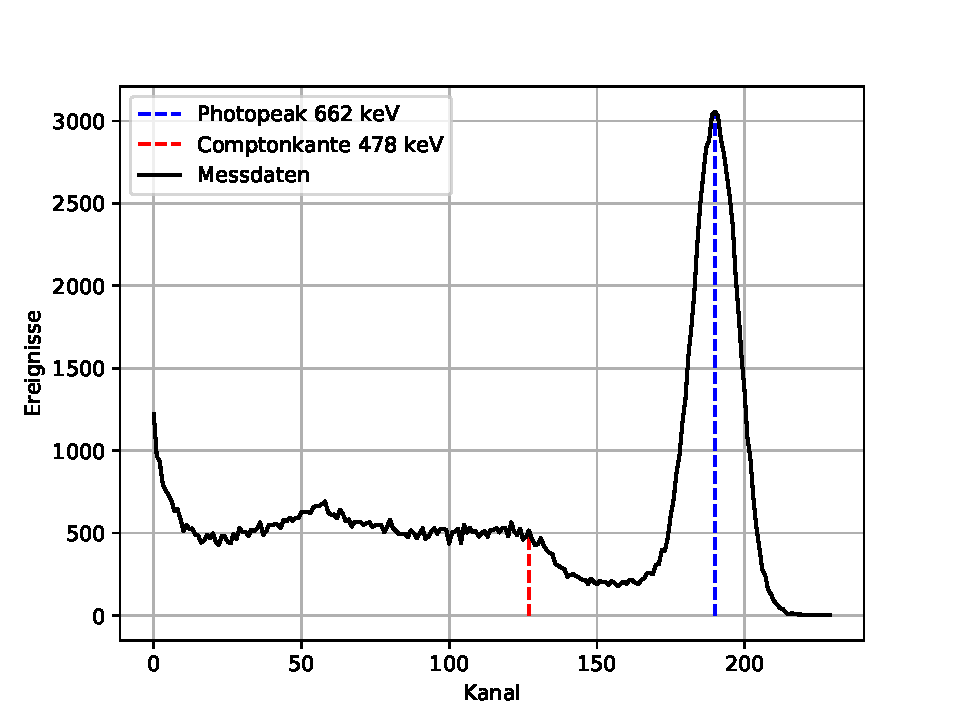
\includegraphics[width=0.8\textwidth]{figure/Leer.pdf}
    \caption{Spektrum des $\ce{^137Cs}$-Strahler ohne Würfel.}
    \label{fig:Leer}
\end{figure}

\subsection{Bestimmung der Absorptionskoeffizienten}

Um die Absorptionskoeffizienten zu bestimmen, müssen zunächst die $I_0$-Werte bestimmt werden. 
Der eigentliche $I_0$-Wert wird bestimmt, indem der Inhalt des Photopeak einer Messung ohne 
Absorbermaterial berechnet wird. Dafür wird ein Bereich um den Photopeak markiert und das Auswertungsprogramm summiert die einzelnen 
Kanäle in dem Bereich auf.
Dieser Bereich wird für die gesamte Messung nicht verändert. Um die Auswertung zu erleichtern wird in diesem Fall
der $I_0$-Wert nicht mit einer Leermessung bestimmt, sondern mit der Aluminiumhülle, da diese für jeden 
Würfel gleich ist. Es werden drei 
verschiedene $I_0$-Werte gemessen( Diagonale $D$, Nebendiagonale $ND$ und seitenparallele Grade $SG$).
Die $I_0$-Werte sind in Tabelle \ref{tab:I_0} aufgelistet.

\FloatBarrier
\begin{table}
    \centering
    \caption{Messdaten für die Bestimmung der $I_0$-Werte und die dazugehörigen $I_0$-Werte.}
    \label{tab:I_0}
    \begin{tabular}{c c c c}
        \toprule
        Ausrichtung&Peakinhalt $C$&Zeit $\Delta t \,/\,\SI{}{\second}$&Zählrate $I_0 \,/\,\SI{}{1\per\second}$\\
        \midrule
        $D$ &$\num{10396(300)}$&$\num{126.44}$&$\num{82.2(24)}$\\
        $ND$&$\num{14398(247)}$&$\num{117.90}$&$\num{122.1(21)}$\\
        $SG$&$\num{12927(271)}$&$\num{119.60}$&$\num{108.1(23)}$\\
        \bottomrule
    \end{tabular}
\end{table}
\FloatBarrier

\subsubsection{Würfel 2 und 3}

Die beiden Würfel 2 und 3 bestehen aus je einem Material, daher werden nur drei Werte gemessen.
Die Messdaten sind in Tabelle \ref{tab:Würfel_1_2} aufgelistet.

\FloatBarrier
\begin{table}
    \centering
    \caption{Messdaten für die Bestimmung der Absorptionskoeffizienten der Würfel 2 und 3.}
    \label{tab:Würfel_1_2}
    \begin{tabular}{c c c c c c c}
        \toprule
        &\multicolumn{3}{c}{Würfel 2}&\multicolumn{3}{c}{Würfel 3}\\
        \cmidrule(lr){2-4}\cmidrule(lr){5-7}
        Ausrichtung&$C$&$\Delta t \,/\,\SI{}{\second}$&$I \,/\,\SI{}{1\per\second}$&$C$&$\Delta t \,/\,\SI{}{\second}$&$I \,/\,\SI{}{1\per\second}$\\
        \midrule
        $D$ &$\num{5096(109)}$&$\num{300}$&$\num{16.6(5)}$&$\num{19747(237)}$&$\num{210.88}$&$\num{93.6(11)}$\\
        $ND$&$\num{4984(157)}$&$\num{300}$&$\num{16.9(4)}$&$\num{22765(246)}$&$\num{208.98}$&$\num{108.9(12)}$\\
        $SG$&$\num{7662(142)}$&$\num{300}$&$\num{25.5(5)}$&$\num{19147(225)}$&$\num{178.60}$&$\num{107.2(13)}$\\
        \bottomrule
    \end{tabular}
\end{table}
\FloatBarrier

Mit den Gleichungen

\begin{equation*}
    \mu_{\text{j}}= \frac{\log{\left(\frac{I_0}{I_\text{j}}\right)}}{d_{\text{j}}}
\end{equation*} 

und den Messdaten aus Tabelle \ref{tab:Würfel_1_2} und \ref{tab:I_0} können die Absorptionskoeffizienten bestimmt werden. 
Die Weglängen $d_{\text{j}}$ betragen

\begin{gather*}
    d_{D} =\frac{3}{\sqrt{2}}\SI{}{\centi\meter}\\
    d_{ND}=\frac{2}{\sqrt{2}}\SI{}{\centi\meter}\\
    d_{SG}=\SI{3}{\centi\meter}.
\end{gather*}

Die berechneten Absorptionskoeffizienten der beiden Würfel sind in Tabelle \ref{tab:Absorptionskoeffizienten_1_2} aufgelistet.

\FloatBarrier
\begin{table}
    \centering
    \caption{Absorptionskoeffizienten der Würfel 2 und 3, gemittelt und für jede einzelne Ausrichtung.}
    \label{tab:Absorptionskoeffizienten_1_2}
    \begin{tabular}{c c c}
        \toprule
        &Würfel 2&Würfel 3\\
        \cmidrule(lr){2-2}\cmidrule(lr){3-3}
        Ausrichtung&$\mu \,/\,\SI{}{1\per\centi\meter}$&$\mu \,/\,\SI{}{1\per\centi\meter}$\\
        \midrule
        D &$\num{0.466(6)}$&$\num{-0.099(11)}$\\
        ND&$\num{0.565(15)}$&$\num{0.063(5)}$\\
        SG&$\num{0.481(9)}$&$\num{0.003(8)}$\\
        \midrule
        gemittelt&$\num{0.504(6)}$&$\num{0.033(5)}$\\
        \bottomrule
    \end{tabular}
\end{table}
\FloatBarrier

Für den Mittelwert aus Tabelle \ref{tab:Absorptionskoeffizienten_1_2} wird der negative Wert nicht beachtet, da dieser unphysikalisch ist,
worauf in der Diskussion eingegangen wird. Um das Material der Würfel zu bestimmen, wird die relative Abweichung der Absorptionskoeffizienten zu 
den vorgegebenen Materialien bestimmt. Die Absorptionskoeffizienten und die Abweichungen sind in Tabelle \ref{tab:Abweichung23}
aufgelistet.

\FloatBarrier
\begin{table}
    \centering
    \caption{Absorptionskoeffizienten der vorgegebenen Materialien und die relative Abweichung der Würfel zu jedem Material. Die 
    Literaturwerte werden mithilfe der Quellen \cite{Massenkoef} und \cite{Dichte} ermittelt.}
    \label{tab:Abweichung23}
    \begin{tabular}{c c c c}
        \toprule
        &&Würfel 2& Würfel 3\\
        \cmidrule(lr){3-3}\cmidrule(lr){4-4}
        Material&$\mu_{\text{Lit}}\,/\,\SI{}{1\per\centi\meter}$&rel. Abweichung /\%&rel. Abweichung /\%\\
        \midrule
        $\ce{Al}$&$\num{0.211}$&$\num{138.9}$&$\num{84.5}$\\
        $\ce{Pb}$&$\num{1.419}$&$\num{64.5}$&$\num{97.7}$\\
        $\ce{Fe}$&$\num{0.606}$&$\num{16.8}$&$\num{94.6}$\\
        Messing  &$\num{0.638}$&$\num{21.0}$&$\num{94.9}$\\ 
        Delrin   &$\num{0.121}$&$\num{316.7}$&$\num{73.0}$\\
        \bottomrule
    \end{tabular}
\end{table}
\FloatBarrier

Wie an den Abweichungen in Tabelle \ref{tab:Abweichung23} zu sehen ist, wird Würfel 2 mit Eisen und Würfel 3 mit Delrin identifiziert. Auf die 
Identifizierung wird in der Diskussion drauf eingegangen.

\subsubsection{Würfel 4}

Die Teilwürfel aus Würfel 4 bestehen aus verschiedenen Materialien, daher wird die Gleichung \ref{eq6} benötigt.
Die Elemente der diagonalen Gewichtsmatrix $W$ werden mithilfe der Gauß´schen Fehlerfortpflanzung bestimmt.

\begin{align*}
    \sigma_{\text{j}}=& \left(\sqrt{\left(\frac{\sigma_{I_0}}{I_0}\right)^2+ \left(\frac{\sigma_{I_j}}{I_j}\right)^2}\right)\\
    W_{\text{jj}}=& \sigma_{\text{j}}^{-1}
\end{align*}

Die Messdaten für die Bestimmung der Absorptionskoeffizienten sind in Tabelle \ref{tab:Messdaten_Würfel4} aufgelistet.

\FloatBarrier
\begin{table}
    \centering
    \caption{Messdaten und die damit bestimmten Elemente der Gewichtsmatrix für die Bestimmung der Absorptionskoeffizienten des Würfels 4. Jede Ausrichtung wurde $\SI{300}{\second}$ lang gemessen. Die Ausrichtungen sind analog zu Abbildung \ref{abb2} benannt und durchgeführt worden. }
    \label{tab:Messdaten_Würfel4}
    \begin{tabular}{c c c c c}
        \toprule
        Ausrichtung $j$&$C$&$I\,/\,\SI{}{1\per\second}$&$\sigma_{\text{j}}$&$W_{\text{jj}}$\\
        \midrule
        $\num{1}$&$\num{24609}$&$\num{82.0}$ &$\num{0.031}$&$\num{32.2}$\\
        $\num{2}$&$\num{16380}$&$\num{54.6}$ &$\num{0.022}$&$\num{44.6}$\\
        $\num{3}$&$\num{25913}$&$\num{86.4}$ &$\num{0.031}$&$\num{32.5}$\\
        $\num{4}$&$\num{16964}$&$\num{56.5}$ &$\num{0.026}$&$\num{38.6}$\\
        $\num{5}$&$\num{17465}$&$\num{58.2}$ &$\num{0.026}$&$\num{39.1}$\\
        $\num{6}$&$\num{14876}$&$\num{49.6}$ &$\num{0.028}$&$\num{35.7}$\\
        $\num{7}$&$\num{21195}$&$\num{70.6}$ &$\num{0.032}$&$\num{31.2}$\\
        $\num{8}$&$\num{16389}$&$\num{54.6}$ &$\num{0.023}$&$\num{43.6}$\\
        $\num{9}$&$\num{23458}$&$\num{78.2}$ &$\num{0.032}$&$\num{31.7}$\\
        $\num{10}$&$\num{12895}$&$\num{43.0}$&$\num{0.031}$&$\num{32.4}$\\
        $\num{11}$&$\num{15569}$&$\num{51.9}$&$\num{0.027}$&$\num{36.9}$\\
        $\num{12}$&$\num{17778}$&$\num{59.3}$&$\num{0.025}$&$\num{39.4}$\\
        \bottomrule
    \end{tabular}
\end{table}
\FloatBarrier

Mit den Messdaten \ref{tab:Messdaten_Würfel4} und der Gleichung \ref{eq6} können die 
Absorptionskoeffizienten $\vec{\mu}$ bestimmt werden. Die Elemente von $\vec{\mu}$ sind in Tabelle \ref{tab:Würfel4_mu} 
aufgelistet, sowie die niedrigste relative Abweichung zu den Literaturwerten der möglichen Stoffe. Da die 
Würfel in Würfel 4 aus den Materialien von Würfel 2 und 3 bestehen soll, werden die Daten für Eisen und Delrin zusätlich angegeben.

\FloatBarrier
\begin{table}
    \centering
    \caption{Absorptionskoeffizienten der einzelnen Würfel in Würfel 4 und die relativen Abweichungen zu den Materialien. Die relativen Abweichungen (rel. Abw.) sind in \% angegeben.}
    \label{tab:Würfel4_mu}
    \begin{tabular}{c c c c c}
        \toprule
        Würfel $j$&$\mu_{\text{j}} \,/\,\SI{}{1\per\centi\meter}$&niedrigste rel. Abw. (Material)& rel. Abw. $\ce{Fe}$&rel. Abw. Delrin\\
        \midrule
        $\num{1}$ &$\num{0.137}$&$\num{13.5}$ (Delrin)&$\num{77.3}$&$\num{13.5}$\\
        $\num{2}$ &$\num{0.119}$&$\num{1.6}$ (Delrin)&$\num{80.3}$&$\num{1.6}$\\
        $\num{3}$ &$\num{0.269}$&$\num{27.6}$ (Al)&$\num{55.6}$&$\num{122.5}$\\
        $\num{4}$ &$\num{0.063}$&$\num{47.7}$ (Delrin)&$\num{89.6}$&$\num{47.7}$\\
        $\num{5}$ &$\num{0.206}$&$\num{2.5}$ (Al)&$\num{66.0}$&$\num{70.1}$\\
        $\num{6}$ &$\num{0.081}$&$\num{33.3}$ (Delrin)&$\num{86.7}$&$\num{33.3}$\\
        $\num{7}$ &$\num{0.225}$&$\num{6.5}$ (Al)&$\num{62.9}$&$\num{85.7}$\\
        $\num{8}$ &$\num{0.064}$&$\num{47.5}$ (Delrin)&$\num{89.5}$&$\num{47.5}$\\
        $\num{9}$ &$\num{0.359}$&$\num{40.8}$ (Fe)&$\num{40.8}$&$\num{196.6}$\\
        \bottomrule
    \end{tabular}
\end{table}
\FloatBarrier

Auf die Glaubwürdigkeit der Identifizierung wird in der Diskussion eingegangen.
\newpage